%
% tikztemplate.tex
%
% (c) 2018 Prof Dr Andreas Müller, Hochschule Rapperswil
%
\documentclass[tikz,12pt]{standalone}
\usepackage{times}
\usepackage{amsmath}
\usepackage{txfonts}
\usepackage[utf8]{inputenc}
\usepackage{graphics}
\usepackage{color}
\usepackage{pifont}
\usetikzlibrary{arrows,intersections,math,calc}
\begin{document}

\def\punkt#1{
        \fill[color=white] #1 circle[radius=0.08];
        \draw[color=red] #1 circle[radius=0.08];
}

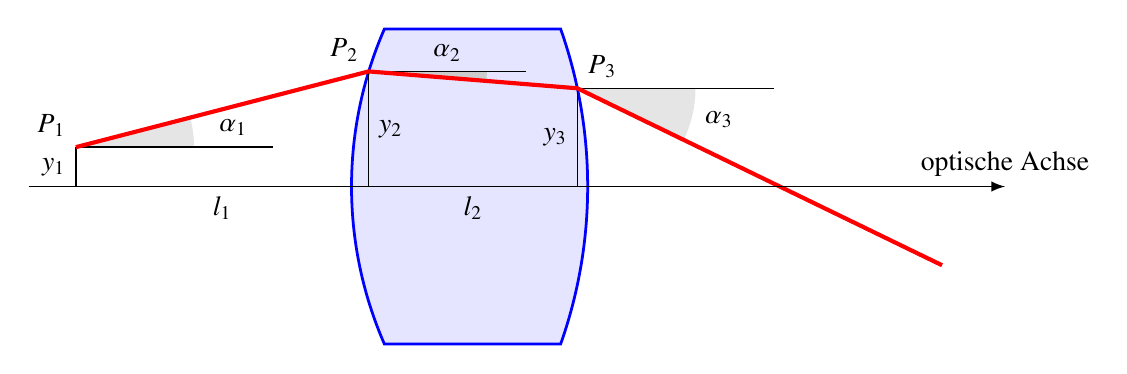
\begin{tikzpicture}[>=latex,thick]

\def\rone{6}
\def\rtwo{5}
\def\aone{19.471}
\def\atwo{23.578}
\def\sone{1}
\def\stwo{-2}

\fill[color=blue!10] ({\stwo+\rtwo-\rtwo*cos(\atwo)},{\rtwo*sin(\atwo)})
	arc ({180-\atwo}:{180+\atwo}:\rtwo)
	--
	({\sone-\rone+\rone*cos(\aone)},{-\rone*sin(\aone)})
	arc ({-\aone}:{\aone}:\rone)
	--cycle;

\draw[color=blue,line width=1pt]
	({\stwo+\rtwo-\rtwo*cos(\atwo)},{\rtwo*sin(\atwo)})
		arc ({180-\atwo}:{180+\atwo}:\rtwo)
	--
	({\sone-\rone+\rone*cos(\aone)},{-\rone*sin(\aone)})
		arc ({-\aone}:{\aone}:\rone)
	--cycle;

\def\bone{12}
\def\btwo{17}

\fill[color=gray!20] (-5.5,0.5)--(-4,0.5) arc (0:14:1.5)--cycle;
\node at (-5.5,0.25) [left] {$y_1$};
\draw[line width=0.5pt] (-5.5,0.0)--(-5.5,0.5);
\draw[line width=0.5pt] (-5.5,0.5)--(-3,0.5);

\node at (-3.5,0.75) {$\alpha_1$};

\fill[color=gray!40]
	({\stwo+\rtwo-\rtwo*cos(\btwo)},{\rtwo*sin(\btwo)})
	--
	({\stwo+\rtwo-\rtwo*cos(\btwo)+1.5},{\rtwo*sin(\btwo)})
	arc (0:-4:1.5)--cycle;
\node at ({\stwo+\rtwo-\rtwo*cos(\btwo)+1},{\rtwo*sin(\btwo)})
	[above] {$\alpha_2$};
\draw[line width=0.5pt]
	({\stwo+\rtwo-\rtwo*cos(\btwo)},{\rtwo*sin(\btwo)})
	--
	({\stwo+\rtwo-\rtwo*cos(\btwo)},0);
\draw[line width=0.5pt]
	({\stwo+\rtwo-\rtwo*cos(\btwo)},{\rtwo*sin(\btwo)})
	--
	({\stwo+\rtwo-\rtwo*cos(\btwo)+2.0},{\rtwo*sin(\btwo)});
\node at ({\stwo+\rtwo-\rtwo*cos(\btwo)},{\rtwo*sin(\btwo)/2})
	[right] {$y_2$};


\fill[color=gray!20]
	({\sone-\rone+\rone*cos(\bone)},{\rone*sin(\bone)})
	--
	({\sone-\rone+\rone*cos(\bone)+1.5},{\rone*sin(\bone)})
	arc (0:-27:1.5)--cycle;
\node at ({\sone-\rone+\rone*cos(\bone)+1.8},{\rone*sin(\bone)-0.4})
	{$\alpha_3$};
\draw[line width=0.5pt]
	({\sone-\rone+\rone*cos(\bone)},{\rone*sin(\bone)})
	--
	({\sone-\rone+\rone*cos(\bone)},0);
\draw[line width=0.5pt]
	({\sone-\rone+\rone*cos(\bone)},{\rone*sin(\bone)})
	--
	({\sone-\rone+\rone*cos(\bone)+2.5},{\rone*sin(\bone)});
\node at ({\sone-\rone+\rone*cos(\bone)},{\rone*sin(\bone)/2})
	[left] {$y_3$};


\draw[line width=1.5pt,color=red]
	(-5.5,0.5)
	--
	({\stwo+\rtwo-\rtwo*cos(\btwo)},{\rtwo*sin(\btwo)})
	--
	({\sone-\rone+\rone*cos(\bone)},{\rone*sin(\bone)})
	--
	(5.5,-1)
	;

\punkt{(-5.5,0.5)}
\punkt{({\stwo+\rtwo-\rtwo*cos(\btwo)},{\rtwo*sin(\btwo)})}
\punkt{({\sone-\rone+\rone*cos(\bone)},{\rone*sin(\bone)})}

\node at (-5.5,0.5)
	[above left] {$P_1$};
\node at ({\stwo+\rtwo-\rtwo*cos(\btwo)},{\rtwo*sin(\btwo)})
	[above left] {$P_2$};
\node at ({\sone-\rone+\rone*cos(\bone)},{\rone*sin(\bone)})
	[above right] {$P_3$};

\draw[->,line width=0.7pt] (-6.1,0)--(6.3,0) coordinate[label={optische Achse}];

\node at ({0.5*(-5.5+\stwo+\rtwo-\rtwo*cos(\btwo))},0)
	[below] {$l_1$};
\node at ({0.5*(\stwo+\rtwo-\rtwo*cos(\btwo)+\sone-\rone+\rone*cos(\bone))},0)
	[below] {$l_2$};

\end{tikzpicture}

\end{document}

